We performed resolution tests for models with [Fe/H] $\in \{-1.2, -0.4, 0.4\}$ and $M \in \{0.9, 1.3, 1.7\}$ using the Brown thermohaline mixing prescription.
We studied a grid of \texttt{mesh\_delta\_coeff} and \texttt{time\_delta\_coeff} values which span from 0.1 to 1.0 over five log-space steps.
We measure $r$ in each of these models, and in Fig.~\ref{Fig:resolution_test} we plot the absolute value of the relative error between that $r$ value and the reference $r_{\rm ref}$ value reported for that case in Fig.~\ref{fig:mesa_r_spread}.
We calculate the relative error to be $1 - r/r_{\rm{ref}}$.

We find that small values of the mesh coefficient combined with large values of the time coefficient result in large errors.
This occurs because the front of the thermohaline zone, and sometimes the full thermohaline zone, becomes numerically unstable, and large oscillations in $R_0$ lead to large errors in the $r$ calculation.
Furthermore, we find that when the thermohaline front is not properly numerically resolved, it does not propagate upwards in mass coordinate and connect with the convective shell.


\begin{figure*}[!tb]
\begin{center}
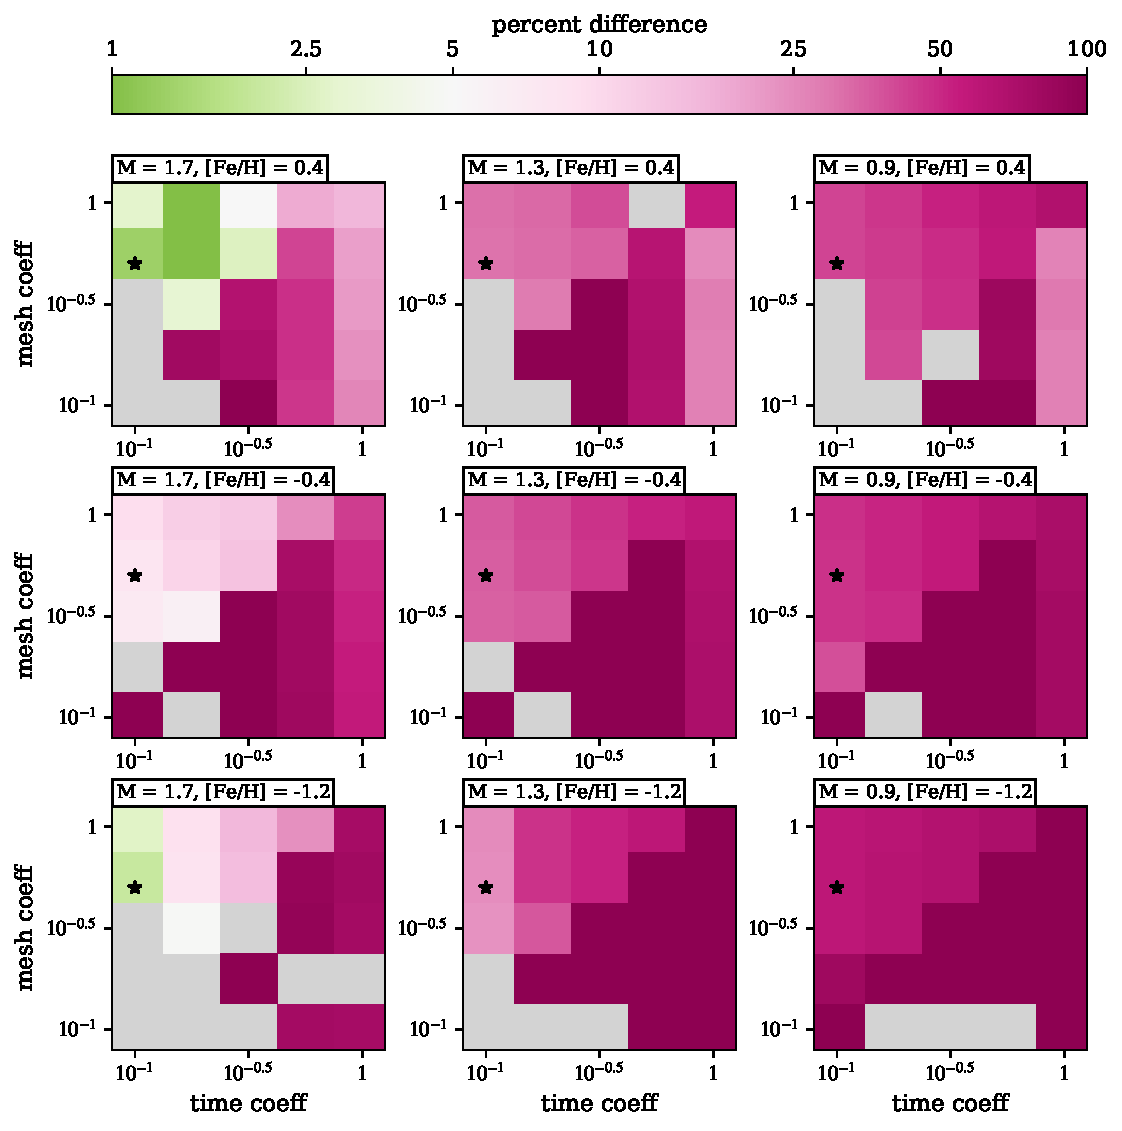
\includegraphics[width=\textwidth]{resolution_test.pdf}
\caption{
    We plot the percent difference between the measured value of the reduced density ratio $r$ for a 5x5 resolution grid of MESA models with respect to the values reported in Fig.~\ref{fig:mesa_r_spread}.
    We study values of \texttt{mesh\_delta\_coeff} and \texttt{time\_delta\_coeff} each in five log-space steps between 0.1 and 1.
    We perform these resolution tests for a 3x3 grid of mass and metallicity with $M \in [0.9, 1.3, 1.7]$ and [Fe/H]$ \in [-1.2, -0.4, 0.4]$.
    Each colored grid in this figure represents a 5x5 resolution test at one value of $M$ and [Fe/H] as reported in the text label above the grid.
    The resolution of the grids of simulations presented in Fig.~\ref{fig:mesa_r_spread} are marked by black stars.
    Points whose percent difference from the reported values are colored in green, while points with larger percent difference are colored in red.
    }
\label{Fig:resolution_test}
\end{center}
\end{figure*}